\documentclass[journal,twoside,print]{ieeecolor}

\usepackage{generic}
\usepackage{cite}
\usepackage{amsmath,amssymb,amsfonts}
\usepackage{booktabs}
\usepackage{graphicx}
\usepackage{microtype}
\usepackage{tabularx}
\usepackage{textcomp}
\usepackage{url}
\usepackage{bm}
\usepackage{hyperref}
\hypersetup{hidelinks}

\def\BibTeX{{\rm B\kern-.05em{\sc i\kern-.025em b}\kern-.08em
    T\kern-.1667em\lower.7ex\hbox{E}\kern-.125emX}}
\def\journalname{IEEE TRANSACTIONS ON MEDICAL IMAGING}
\def\refname{References}
\emergencystretch=1.5em

\makeatletter
\def\thebibliography#1{\section*{\refname}%
    \addcontentsline{toc}{section}{\refname}%
    \footnotesize \vskip 0.3\baselineskip plus 0.1\baselineskip minus 0.1\baselineskip%
    \list{\@biblabel{\@arabic\c@enumiv}}%
    {\settowidth\labelwidth{\@biblabel{#1}}%
    \leftmargin\labelwidth
    \advance\leftmargin\labelsep\relax
    \itemsep 0pt plus 0pt\relax%
    \usecounter{enumiv}%
    \let\p@enumiv\@empty
    \renewcommand\theenumiv{\@arabic\c@enumiv}}%
    \let\@IEEElatexbibitem\bibitem%
    \def\bibitem{\@IEEEbibitemprefix\@IEEElatexbibitem}%
    \def\newblock{\hskip .11em plus .33em minus .07em}%
    \if@technote\sloppy\clubpenalty4000\widowpenalty4000\interlinepenalty100%
    \else\sloppy\clubpenalty4000\widowpenalty4000\interlinepenalty500\fi%
    \sfcode`\.=1000\relax}
\let\endthebibliography=\endlist
\makeatother

\newcommand{\Tzero}{\ensuremath{T_0}}
\newcommand{\Tone}{\ensuremath{T_1}}
\newcommand{\Ttwo}{\ensuremath{T_2}}
\newcommand{\Tthree}{\ensuremath{T_3}}
\newcommand{\ftv}{\mathrm{FTV}}
\newcommand{\calibrationtag}{\textsc{Endpoint+Active}}
\newcommand{\modeltag}{\textsc{Hybrid-Edge} $k=8$}

\begin{document}

\title{Endpoint-Calibrated Graph-Native Tumor-State Forecasting with Probabilistic Functional Tumor Volume Readouts in Breast DCE-MRI}

\author{Iris Seaman, Tamer Oraby, and Murad Moqbel
\thanks{This work used de-identified breast DCE-MRI resources distributed
through The Cancer Imaging Archive. No external funding is reported for this
analysis.}
\thanks{Iris Seaman is with the Department of Computer Science, College of
Engineering and Computer Science, The University of Texas Rio Grande Valley,
Edinburg, TX 78539 USA (e-mail: iris.seaman01@utrgv.edu).}
\thanks{Tamer Oraby is with the School of Mathematical and Statistical
Sciences, College of Sciences, The University of Texas Rio Grande Valley,
Edinburg, TX 78539 USA (e-mail: tamer.oraby@utrgv.edu).}
\thanks{Murad Moqbel is with the Department of Information Systems, Robert C.
Vackar College of Business and Entrepreneurship, The University of Texas Rio
Grande Valley, Edinburg, TX 78539 USA (e-mail: murad.moqbel@utrgv.edu).}}

\markboth
{\hskip25pc IEEE TRANSACTIONS ON MEDICAL IMAGING}
{Seaman \MakeLowercase{\textit{et al.}}: Endpoint-Calibrated Graph-Native Tumor-State Forecasting}

\maketitle

\begin{abstract}
Serial dynamic contrast-enhanced magnetic resonance imaging during neoadjuvant
breast cancer therapy provides repeated measurements of tumor burden, but most
forecasting pipelines collapse this sequence to scalar functional tumor volume.
This study presents endpoint calibration for graph-native probabilistic
tumor-state forecasting, with functional tumor volume treated as a calibrated
readout from the predicted graph rather than the only forecasted object. Each
tumor is represented as a registration-consistent supervoxel graph, a
scheduled-sampling message-passing forecaster predicts regional motion,
imaging-feature evolution, and active status, and endpoint calibration aligns
the graph rollout with future functional tumor volume. Empirical residual
Monte Carlo simulation then converts the graph center into patient-level
predictive distributions.
Controlled synthetic graph tumors test when neighborhood information should
help, showing that graph message passing is most useful when local
neighborhoods reveal hidden spatial response structure. On 758 held-out
patients from the I-SPY2 and ACRIN graph-bearing breast magnetic resonance
imaging cohort, the final hybrid-edge model reduced deterministic functional
tumor volume error from 12.88 mL to 4.63 mL, Monte Carlo mean error from
15.26 mL to 5.56 mL, and conformal 90\% interval width from 59.51 mL to
22.38 mL, while improving raw 90\% coverage from 0.766 to 0.877. The model
also preserved sampled tumor-cloud geometry and identified low residual imaging
burden at the final visit with area under the receiver operating characteristic
curve 0.957. These results support structured longitudinal tumor-state
forecasting with separate graph-dynamic, endpoint-calibration, and
residual-uncertainty layers.
\end{abstract}

\begin{IEEEkeywords}
Breast dynamic contrast-enhanced magnetic resonance imaging, conformal
prediction, functional tumor volume, graph neural networks, longitudinal
imaging, Monte Carlo simulation, uncertainty calibration.
\end{IEEEkeywords}

\section{Introduction}
\label{sec:intro}

\IEEEPARstart{S}{erial} dynamic contrast-enhanced magnetic resonance imaging
(DCE-MRI) during neoadjuvant breast cancer therapy creates a longitudinal
forecasting problem: given the tumor observed so far, estimate future active
burden and the uncertainty around that burden. I-SPY established serial breast
MRI as a response-monitoring substrate for adaptive neoadjuvant trials
\cite{barker2009ispy2}, and functional tumor volume (FTV) became a central
quantitative MRI biomarker for response and recurrence risk
\cite{hylton2012ispy,hylton2016ftv,li2020ispy2mri,onishi2023ftvvariation}.
Public I-SPY2 and ACRIN-6698 resources distributed through The Cancer Imaging
Archive make the forecasting problem testable at cohort scale
\cite{tciaispy2,tciaacrin6698}.

Most predictive imaging pipelines reduce the serial tumor state to a scalar
endpoint or a response label. That is clinically useful, but it discards the
regional organization visible in DCE-MRI: local enhancement, washout, necrosis,
boundary motion, and segmentation uncertainty can vary across the tumor. A
graph of transported supervoxel regions gives each local region its own state
while preserving spatial relationships. The forecasting question becomes how
regional tumor states move, change enhancement, and remain active or become
inactive over future visits.

This paper studies a layered alternative to scalar-only FTV regression. A
scheduled-sampling graph forecaster rolls a registration-consistent tumor graph
forward in time; endpoint calibration aligns the graph rollout with observed
FTV and active tumor burden; empirical residual Monte Carlo (MC) then converts
the calibrated center into patient-level FTV distributions. This separates
three properties that are often conflated: spatial tumor-state plausibility,
endpoint burden calibration, and predictive-distribution calibration.

The contribution is threefold. First, the method forecasts a graph-native
future tumor state rather than only a scalar FTV value. Second, controlled
synthetic graph tumors identify when message passing should help: local
neighborhoods must carry response information not fully visible from each
node's own features. Third, held-out I-SPY2/ACRIN experiments show that
endpoint calibration and edge-aware neighborhoods substantially improve FTV
error, interval sharpness, coverage, and graph-state burden while preserving
sampled tumor-cloud geometry. Strong scalar and hybrid FTV controls are also
reported to define the boundary of the claim. Rather than claiming universal
graph superiority, the study asks when graph structure is useful, when scalar
readouts remain sufficient, and where uncertainty calibration exposes
safety-relevant limits.

\section{Related Work and Positioning}
\label{sec:related}

Longitudinal breast MRI response models have used handcrafted MRI features,
radiomics, convolutional models, transformers, and temporal fusion networks to
predict pathologic complete response or related response endpoints
\cite{li2020ispy2mri,huang2023longitudinal,tang2025sti}. These studies
motivate serial MRI representation learning, but they usually return a label or
scalar endpoint rather than a future spatial tumor state. Digital twin work is
the closest conceptual neighbor: image-calibrated mathematical models can
simulate patient-specific breast tumor response under treatment
\cite{weis2013mechanically,wu2022digitalmodels,wu2025digitaltwins}. The present
study follows a complementary data-driven route focused on longitudinal MRI
burden forecasting across observed visits.

These neighboring literatures motivate but do not replace the present task.
Response classifiers are evaluated against pathology labels, mechanistic twins
simulate patient-specific response with explicit tumor-growth models, and
scalar FTV models provide strong endpoint readouts. The target here is the
intersection that those approaches do not directly provide: a learned
graph-native future tumor state with a calibrated patient-level FTV
distribution.

Graph neural networks are natural for structured dynamical systems because
message passing can aggregate local relational information
\cite{gilmer2017neural,sanchezgonzalez2018physics}. Scheduled sampling reduces
exposure bias in autoregressive sequence prediction \cite{bengio2015scheduled}.
Here, these ideas are applied to transported tumor supervoxels: nodes represent
local tumor regions, edges represent local spatial or feature-neighborhood
relationships, and the model predicts the next graph state.

The uncertainty layer is empirical rather than Bayesian. Model weights are
fixed after training; uncertainty samples are generated by resampling
held-out residual structure around the deterministic rollout center. The
resulting FTV distributions are evaluated with mean error, coverage, conformal
intervals \cite{angelopoulos2021conformal,romano2019cqr}, and Continuous
Ranked Probability Score (CRPS), a proper score for predictive distributions
\cite{gneiting2007proper}. This makes the paper a probabilistic imaging-burden
forecasting study rather than a response-classification or segmentation study.

\section{Methods and Evaluation Design}
\label{sec:methods}

\subsection{Forecasting Task and Graph Representation}

For patient $p$ and visit $t$, the tumor graph is
$G_p^{(t)}=(V_p^{(t)},E_p^{(t)})$. Each node is a compact baseline tumor
supervoxel produced by Simple Linear Iterative Clustering (SLIC)
\cite{achanta2012slic} and transported to follow-up visits by symmetric
diffeomorphic registration \cite{avants2008symmetric}. Node features are
$\log(1+\mathrm{voxel\ count})$, volume in mL, percent-enhancement mean and
standard deviation, signal-enhancement-ratio mean and standard deviation, and
centroid position after subtracting the visit-level tumor centroid. The active
target records whether the transported supervoxel has tumor support at that
visit.

The forecasted object is a future graph state
$\widehat{G}_{p,t}$ conditioned on observed visits $G_{p,\leq s}$. FTV is read
from that state as
\begin{equation}
\widehat{\ftv}_{p,t} =
\sum_{i\in V_p^{(t)}} \widehat{a}_{p,t,i}\widehat{v}_{p,t,i},
\end{equation}
where $\widehat{a}_{p,t,i}$ is the predicted active probability and
$\widehat{v}_{p,t,i}$ is the predicted node volume. Spatial quality is
therefore evaluated separately from scalar burden by sliced Wasserstein
distance (SWD), Chamfer distance, Dice, and active-node-count error.

\subsection{Graph Rollout, Endpoint Calibration, and MC}

All graph-family models use the same autoregressive local spatial graph
convolution backbone. The forecaster embeds node features into a
64-dimensional hidden state, applies residual message passing with shared
weights, and predicts next-visit displacement, feature change, and active-node
logit. During training, scheduled sampling transitions from teacher-forced
history to self-fed rollouts. The original graph rollout is the geometry-first
baseline.

Endpoint calibration adds losses on aggregate FTV and active-node burden while
retaining the node-level spatial and feature losses. The first calibrated model
uses spatial $k=8$ neighborhoods and is denoted \calibrationtag. The final
retained model, \modeltag, rebuilds neighborhoods dynamically with a hybrid
spatial-feature distance and radial imaging-feature edge attributes. Candidate
neighbors are ranked by an equally weighted normalized blend of spatial and
feature distance, then symmetrized. The retained real-cohort graph uses a
64-dimensional hidden state, two message-passing layers, $k=8$ neighborhoods,
scheduled sampling annealed to 0.5, and endpoint weights
$\lambda_{\ftv}=0.20$ and $\lambda_{\mathrm{act}}=0.05$.

For a rollout ending at visit $t$, the training objective combines local state
losses with endpoint losses,
\begin{equation}
\begin{split}
\mathcal{L} =
&\,\mathcal{L}_{\mathrm{node}}+
\lambda_{\ftv}\left|\widehat{\ftv}_{p,t}-\ftv_{p,t}\right|\\
&+\lambda_{\mathrm{act}}
\left|\sum_i \widehat{a}_{p,t,i}-\sum_i a_{p,t,i}\right|.
\end{split}
\end{equation}
The node term includes feature, displacement, and active-logit losses; the FTV
term centers the scalar endpoint read from the graph; and the active-burden
term prevents scalar FTV calibration from drifting away from the sampled active
state. This design keeps the graph rollout interpretable: the scalar endpoint
is not trained as an unrelated head, but as a readout constrained by predicted
node volume and activity.

After training, the deterministic graph rollout is fixed. Patient-level MC
samples are generated by resampling held-out residuals from matching
conditioning buckets, excluding the target patient's own residuals. The same MC
protocol is used for graph, scalar, and hybrid centers. Scalar controls include
last-observed FTV and regularized temporal FTV centers; the hybrid center fits
an out-of-fold ridge model using the graph prediction, last-observed FTV, and
\Tzero{} FTV.

The edge attributes encode relative displacement and local enhancement/volume
differences. The node loss combines feature, displacement, and active-logit
terms, while endpoint terms are enabled after the configured warmup schedule.
Synthetic graph cohorts are generated under node-local, neighbor-coupled, and
latent spatial-field response mechanisms to test whether message passing helps
only when neighborhoods contain useful response information. Split files,
preprocessing summaries, retained configurations, evaluation scripts, and
figure/table generation code are maintained in the reviewer-facing release
repository. Protected patient-level imaging data are not redistributed.

Each endpoint MC distribution uses 128 residual draws. For graph-family models,
the deterministic rollout also provides a predicted active-probability vector
and node volumes; residual draws perturb the endpoint FTV center and sampled
active burden while preserving the patient-specific graph support. Graph-state
metrics are therefore computed from predicted and observed active supervoxel
clouds, whereas scalar controls are evaluated only on FTV distributions. This
keeps the scalar readout comparison fair without pretending that scalar
baselines produce a future tumor graph.

All reported real-cohort estimates use held-out-patient folds. Residual pools,
conformal calibration, scalar baselines, and hybrid readouts are fit without
using the target patient's held-out residuals. This is important because the
MC distribution can otherwise look calibrated by reusing a patient's own
forecast error. The reported conformal widths are therefore computed after the
same target-patient exclusion rule used for residual sampling.

\begin{figure*}[t]
\centering
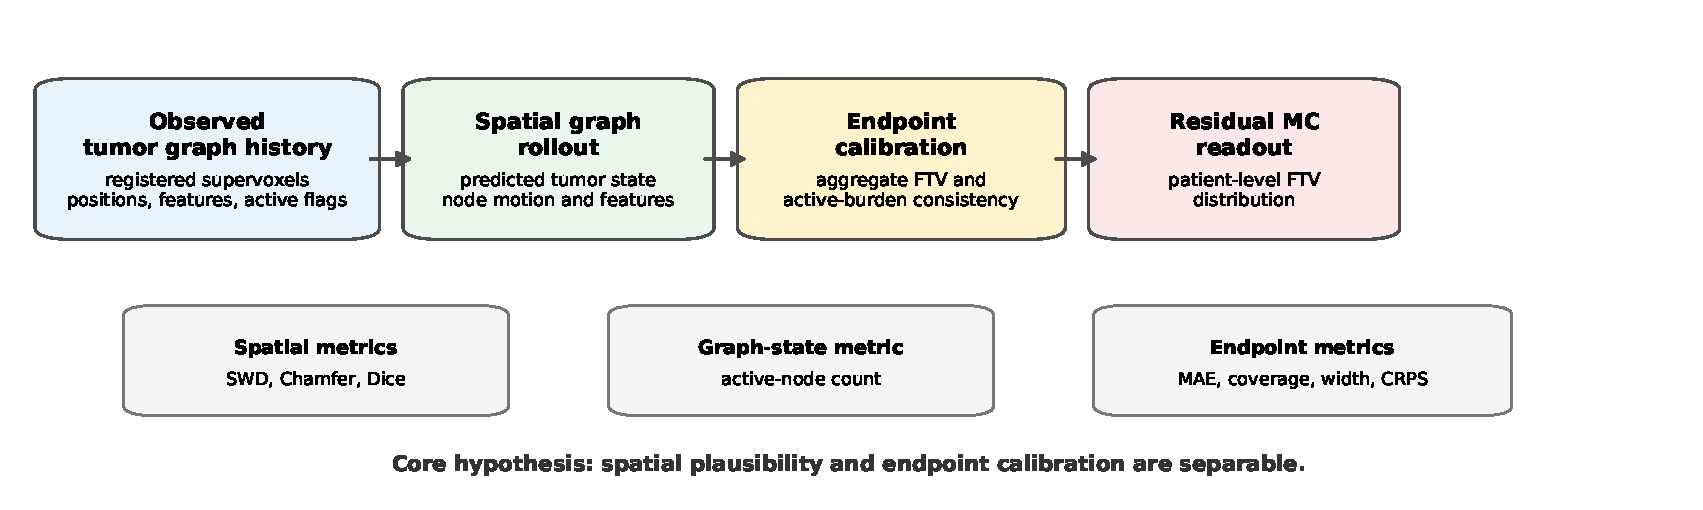
\includegraphics[width=0.88\textwidth]{figures/endpoint_calibrated_spatial_forecasting.pdf}
\caption{End-to-end endpoint-calibrated spatial graph forecasting pipeline.
Serial DCE-MRI visits are converted into a registration-consistent SLIC
supervoxel graph, a hybrid-edge rollout predicts future node motion,
imaging-feature evolution, and active status, FTV is read from predicted
active volume, and residual MC with conformal correction produces the
patient-level predictive distribution. Evaluation keeps endpoint metrics and
graph-state metrics separate.}
\label{fig:ecsf}
\end{figure*}

\subsection{Cohorts, Synthetic Controls, and Metrics}

The real-cohort evaluation uses 758 graph-bearing patients with four
longitudinal DCE-MRI visits across the I-SPY2/ACRIN-derived cohort. Each
patient is evaluated in the fold in which that patient was held out. The
primary real-cohort task is \Tzero$\rightarrow$\Tthree{} FTV forecasting; the
same final-visit target is also evaluated from \Tone{} and \Ttwo{} conditioning.
Primary metrics are deterministic FTV MAE, MC-mean FTV MAE, CRPS, raw 90\%
coverage, and interval width. Secondary metrics include active-node-count
error, SWD, Chamfer distance, Dice, source and subtype stratification, a small
external Breast-MRI-NACT-Pilot stress test, and low/high residual MRI-burden
threshold readouts.

Synthetic graph tumors are generated to test the graph assumption under known
dependence structure before interpreting real-cohort ablations. The node-local
regime makes future response mostly recoverable from each node's own features.
The neighbor-coupled regime makes future response depend partly on local
neighbor state. The latent spatial-field regime drives response from a hidden
smooth regional field observed through noisy local proxies. The synthetic
question is whether message passing improves endpoint and graph-state metrics
when local neighborhoods reveal information that node-local features only
partially observe.

The small external Breast-MRI-NACT-Pilot analysis is treated only as a stress
test of model-family transfer. It uses source-trained graph checkpoints and
source-cohort residual MC calibration on 11 graph-ready external patients. No
NACT residuals are used for recalibration, so the result tests relative
ordering under collection shift rather than powered clinical generalization.

\section{Results}
\label{sec:results}

\subsection{Synthetic Controls Identified When Edges Help}

The synthetic results support a conditional view of message passing. When
response was node-local, the no-edge model remained competitive for scalar FTV.
When response depended on a latent spatial field, \modeltag{} reduced
\Tzero$\rightarrow$\Tthree{} MC-mean FTV MAE by 5.43 mL relative to the no-edge
endpoint model, reduced CRPS by 3.53, narrowed raw 90\% interval width by
24.14 mL, and improved MC Chamfer distance by 0.41 mm
(Table~\ref{tab:synthetic}). The real-cohort experiments therefore test both
endpoint calibration and whether edge design makes neighborhood information
useful in breast MRI graphs.

\begin{table}[t]
\centering
\caption{Synthetic \Tzero$\rightarrow$\Tthree{} mechanism checks. Deltas are
\modeltag{} minus the no-edge endpoint model; negative values are better for
MAE, CRPS, width, and Chamfer.}
\label{tab:synthetic}
\scriptsize
\setlength{\tabcolsep}{3.2pt}
\begin{tabularx}{\columnwidth}{@{}l>{\raggedright\arraybackslash}Xrrrr@{}}
\toprule
Regime & Graph signal & $\Delta$ MC MAE & $\Delta$ CRPS & $\Delta$ width & $\Delta$ Chamfer \\
 & & (mL) & & (mL) & (mm) \\
\midrule
Node-local & Future response readable from node features. & +0.15 & -0.04 & +0.99 & -0.47 \\
Neighbor-coupled & Future response partly depends on local neighbors. & +0.40 & -0.20 & -1.02 & -0.62 \\
Latent field & Hidden smooth response field is observed through noisy node proxies. & -5.43 & -3.53 & -24.14 & -0.41 \\
\bottomrule
\end{tabularx}
\end{table}

\begin{figure*}[t]
\centering
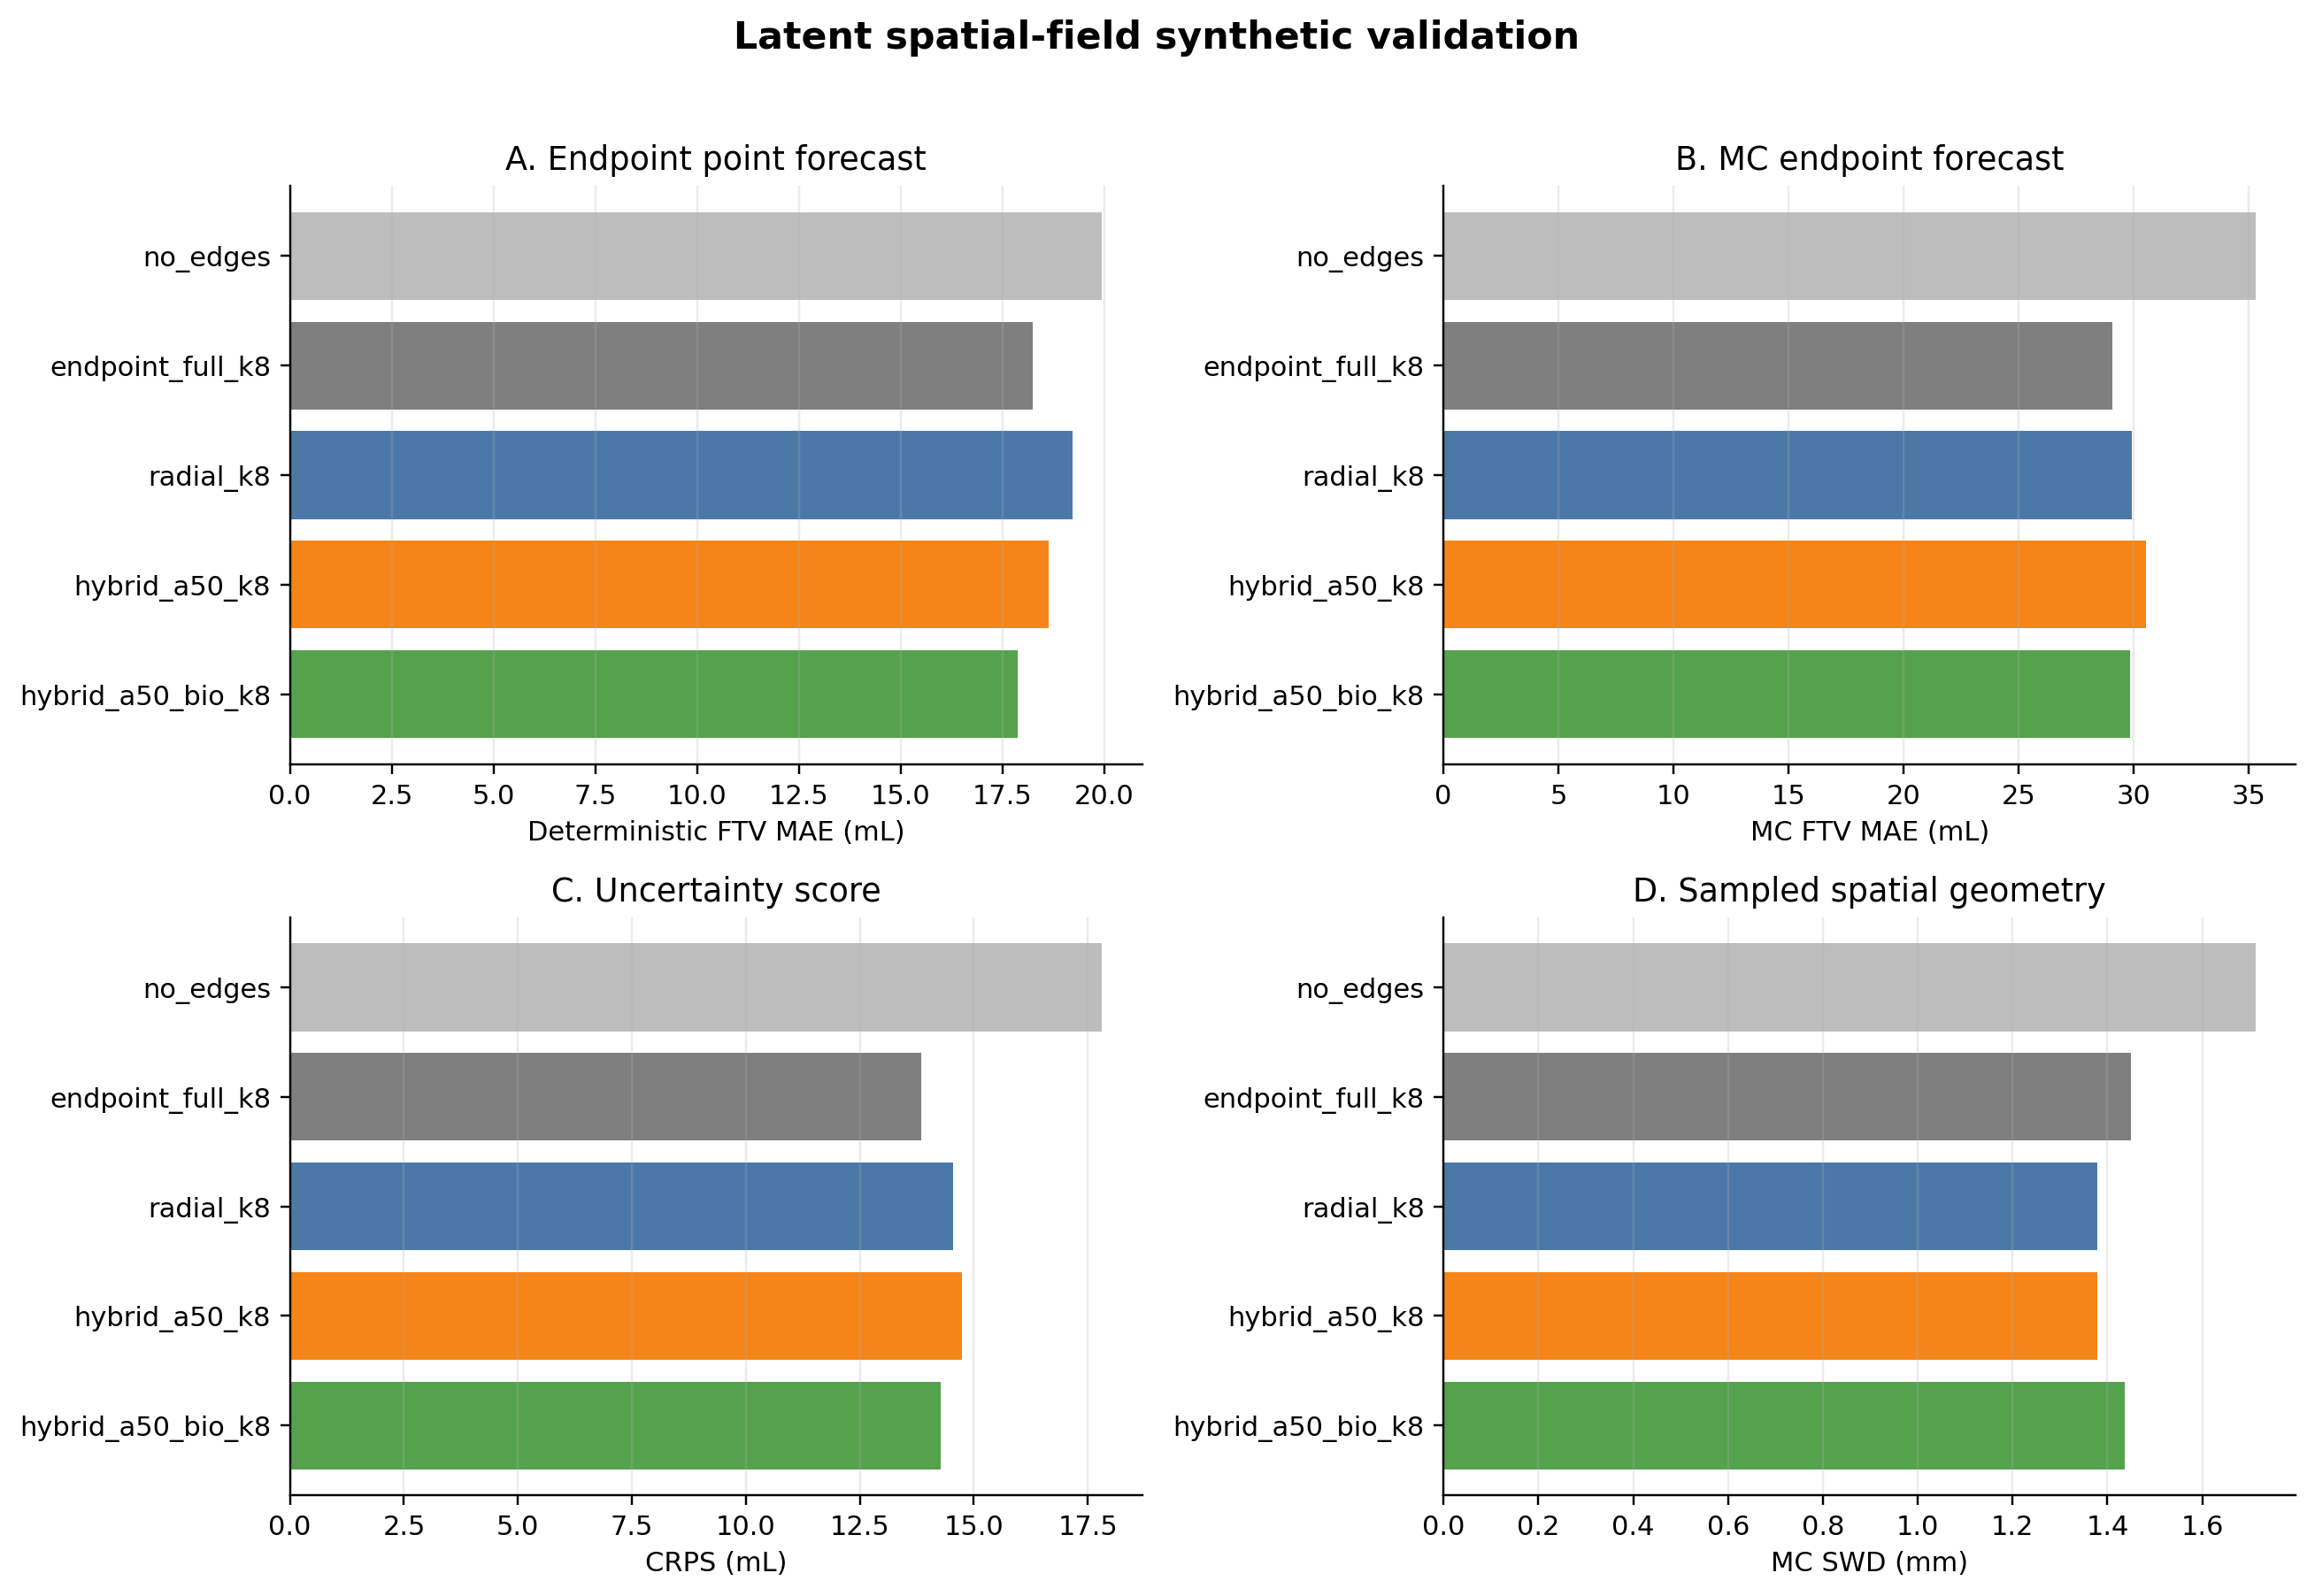
\includegraphics[width=0.86\textwidth]{figures/synthetic_spatial_field_four_panel_summary.png}
\caption{Synthetic latent spatial-field validation. The retained graph becomes
most useful when hidden regional response structure can be denoised through
local neighborhoods, improving endpoint uncertainty and sampled-cloud geometry
relative to the no-edge control.}
\label{fig:syntheticspatialfield}
\end{figure*}

\subsection{Endpoint Calibration and Edge-Aware Graphs Improved the Rollout}

The original graph rollout produced a plausible spatial object but a biased FTV
center. In the held-out \Tzero$\rightarrow$\Tthree{} evaluation, observed mean
FTV was 24.94 mL and the baseline deterministic mean was 12.43 mL, yielding
12.88 mL MAE and -12.51 mL bias. Adding endpoint and active-burden calibration
reduced deterministic MAE to 5.88 mL, bias to -1.73 mL, and active-node-count
absolute error from 58.00 to 1.70 supervoxels, while SWD, Chamfer, and Dice
changed only minimally. This shows that the spatial rollout and endpoint
readout are separable.

Using the same residual MC sampler, endpoint calibration reduced MC-mean FTV
MAE from 15.26 to 7.61 mL, increased raw 90\% coverage from 0.766 to 0.876,
reduced raw interval width from 56.87 to 24.42 mL, reduced conformal 90\%
interval width from 59.51 to 27.95 mL, and reduced CRPS from 8.35 to 5.16.
The paired MC-mean MAE reduction was 7.65 mL (95\% CI: 7.11--8.20).

The final edge-aware graph further improved the graph-family tradeoff. Compared
with the no-edge endpoint model, \modeltag{} lowered deterministic FTV MAE by
0.65 mL, MC-mean FTV MAE by 1.02 mL, CRPS by 0.56, raw interval width by
3.67 mL, conformal width by 4.12 mL, and MC Chamfer by 0.043 mm. The radial
imaging-feature model had the lowest scalar graph MC-mean MAE by a small
margin, but \modeltag{} was retained because it gave the strongest balance of
coverage, conformal width, and sampled-cloud geometry.

\begin{table*}[t]
\centering
\caption{\Tzero$\rightarrow$\Tthree{} main comparison. Width is raw 90\%
interval width for rows with MC samples. Active error is MC active-node-count
absolute error; scalar rows do not produce graph-native state outputs.}
\label{tab:maincomparison}
\scriptsize
\setlength{\tabcolsep}{3.0pt}
\begin{tabular}{lrrrrrrrr}
\toprule
Model & Det. MAE & MC MAE & CRPS & Raw cov. & Raw width & Active err. & MC SWD & MC Chamfer \\
 & (mL) & (mL) & & & (mL) & (SV) & (mm) & (mm) \\
\midrule
Original graph rollout & 12.88 & 15.26 & 8.35 & 0.766 & 56.87 & 40.78 & 1.320 & 3.656 \\
\calibrationtag{} graph & 5.88 & 7.61 & 5.16 & 0.876 & 24.42 & 2.69 & 1.207 & 3.485 \\
No-edge endpoint graph & 5.28 & 6.59 & 4.56 & 0.871 & 22.87 & 2.69 & 1.209 & 3.491 \\
Radial MRI-feature graph & 4.62 & 5.52 & 3.95 & 0.872 & 20.05 & 2.66 & 1.177 & 3.457 \\
\textbf{\modeltag{} graph} & \textbf{4.63} & \textbf{5.56} & \textbf{4.00} & \textbf{0.877} & \textbf{19.21} & \textbf{2.74} & \textbf{1.172} & \textbf{3.449} \\
Last-observed scalar MC & 4.81 & 4.82 & 3.76 & 0.898 & 18.60 & -- & -- & -- \\
Hybrid graph+scalar MC & 4.48 & 4.50 & 3.71 & 0.897 & 18.20 & -- & -- & -- \\
\bottomrule
\end{tabular}
\end{table*}

Figure~\ref{fig:qualrollout} shows two held-out graph-state diagnostics with
nontrivial final burden, one from each source collection. These examples are
not used as cohort-level performance evidence. They show the observed baseline
and final tumor graphs, exact retained-model graph-state metrics at
\Tthree{}, and the endpoint MC distribution for the same forecast. This makes
the graph-native object visible while Tables~\ref{tab:maincomparison}
and~\ref{tab:robustness} carry the aggregate evidence.

\begin{figure*}[t]
\centering
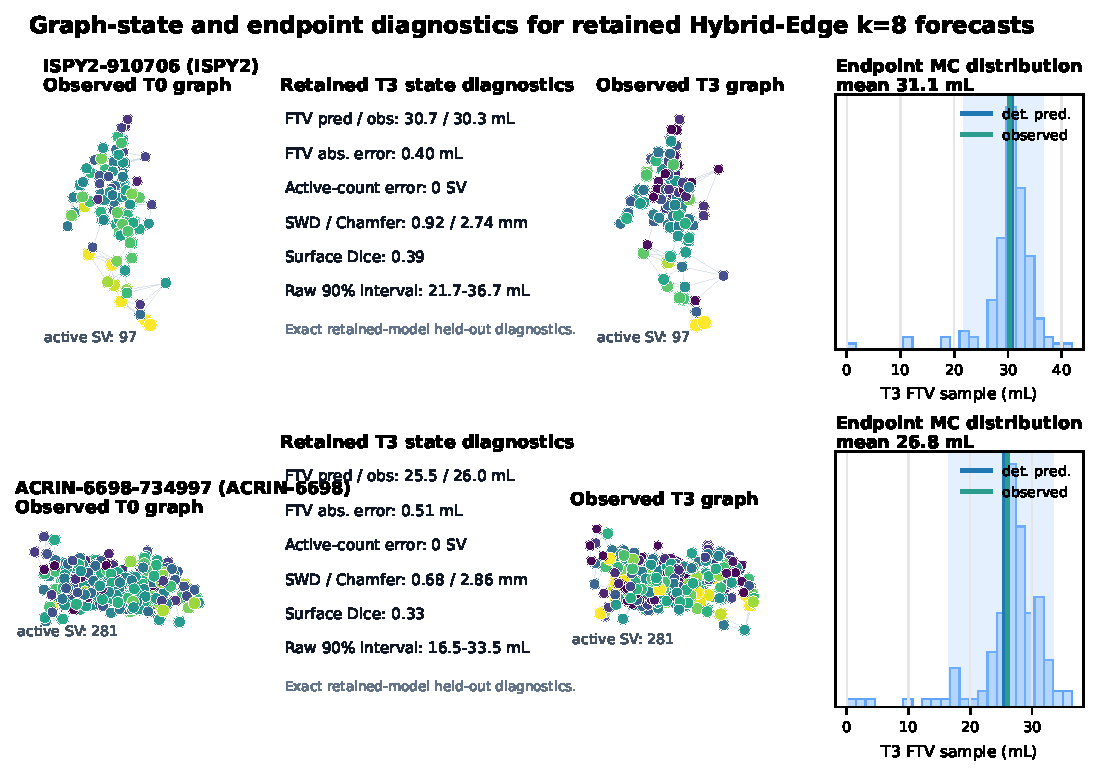
\includegraphics[width=0.92\textwidth]{figures/ispy2_two_patient_rollout_static.pdf}
\caption{Held-out graph-state and endpoint diagnostics from the retained
\modeltag{} graph. Each row shows observed \Tzero{} and \Tthree{} active
supervoxel graphs, exact retained-model \Tthree{} graph-state diagnostics
(FTV error, active-count error, SWD, Chamfer, and surface Dice), and the MC
final-visit FTV distribution.}
\label{fig:qualrollout}
\end{figure*}

The scalar controls define the readout boundary of the contribution. A
last-observed FTV center with out-of-fold residual MC achieved 4.82 mL MC-mean
MAE, 0.898 raw coverage, and 3.76 CRPS. The hybrid graph-plus-scalar center
achieved 4.50 mL MC-mean MAE and 3.71 CRPS. Thus, scalar or hybrid calibration
is strongest when the requested output is only final FTV. The graph rollout
supplies a different object: a structured tumor-state forecast with active-node
dynamics, sampled-cloud geometry, and a calibrated endpoint readout.

\begin{figure*}[t]
\centering
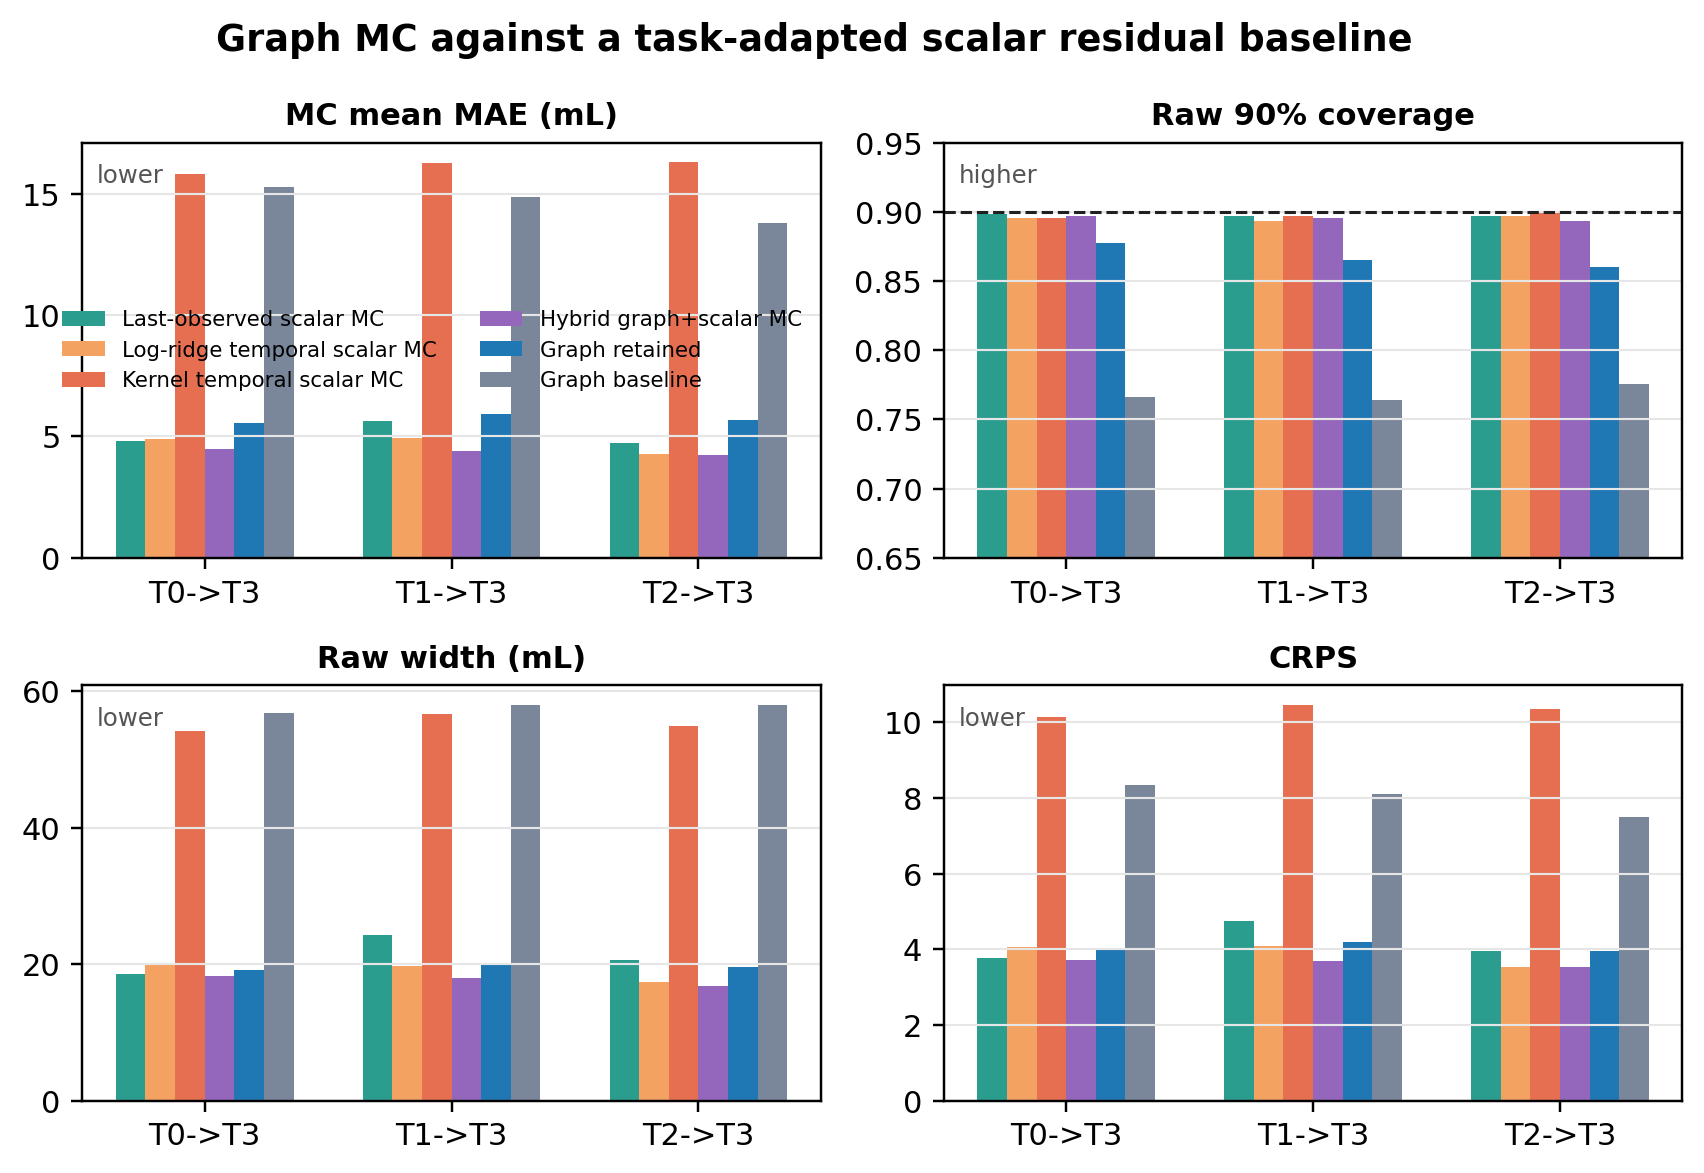
\includegraphics[width=0.88\textwidth]{figures/scalar_vs_graph_mc_t3.png}
\caption{Scalar, graph, and hybrid residual MC controls for final-visit FTV.
Scalar temporal baselines use observed FTV history and metadata before applying
out-of-fold residual MC. The hybrid model combines the graph center with
scalar FTV history, showing that scalar readout calibration and graph-native
state forecasting answer related but distinct questions.}
\label{fig:scalarhybrid}
\end{figure*}

\begin{figure}[t]
\centering
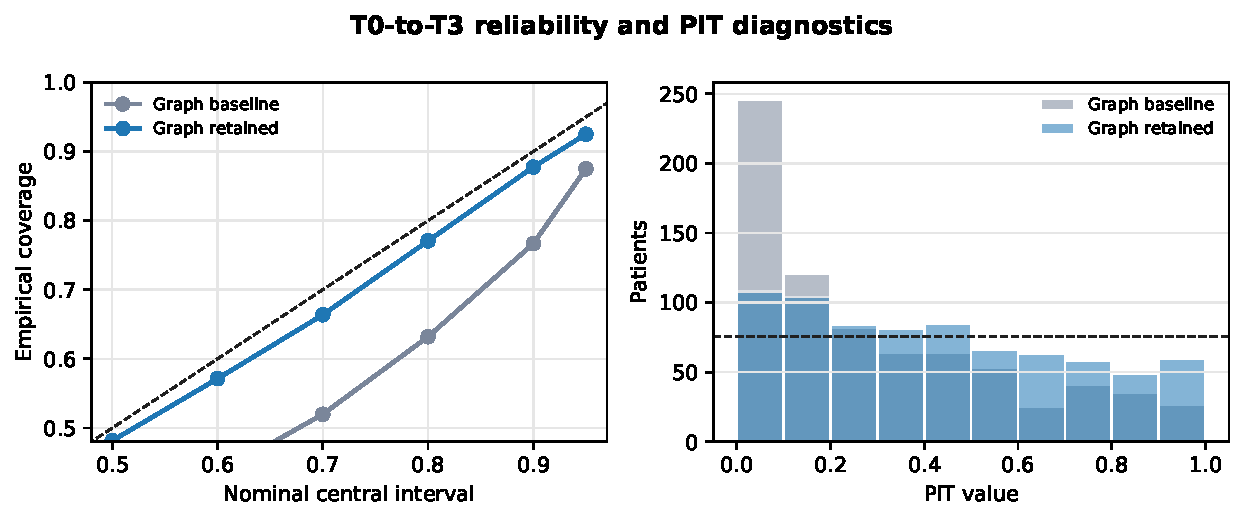
\includegraphics[width=\columnwidth]{figures/reliability_pit_t0t3.pdf}
\caption{\Tzero$\rightarrow$\Tthree{} reliability and PIT diagnostics. The
retained graph improves central-interval coverage across nominal levels and
reduces boundary concentration in the PIT distribution relative to the original
graph rollout.}
\label{fig:reliabilitypit}
\end{figure}

\begin{figure*}[t]
\centering
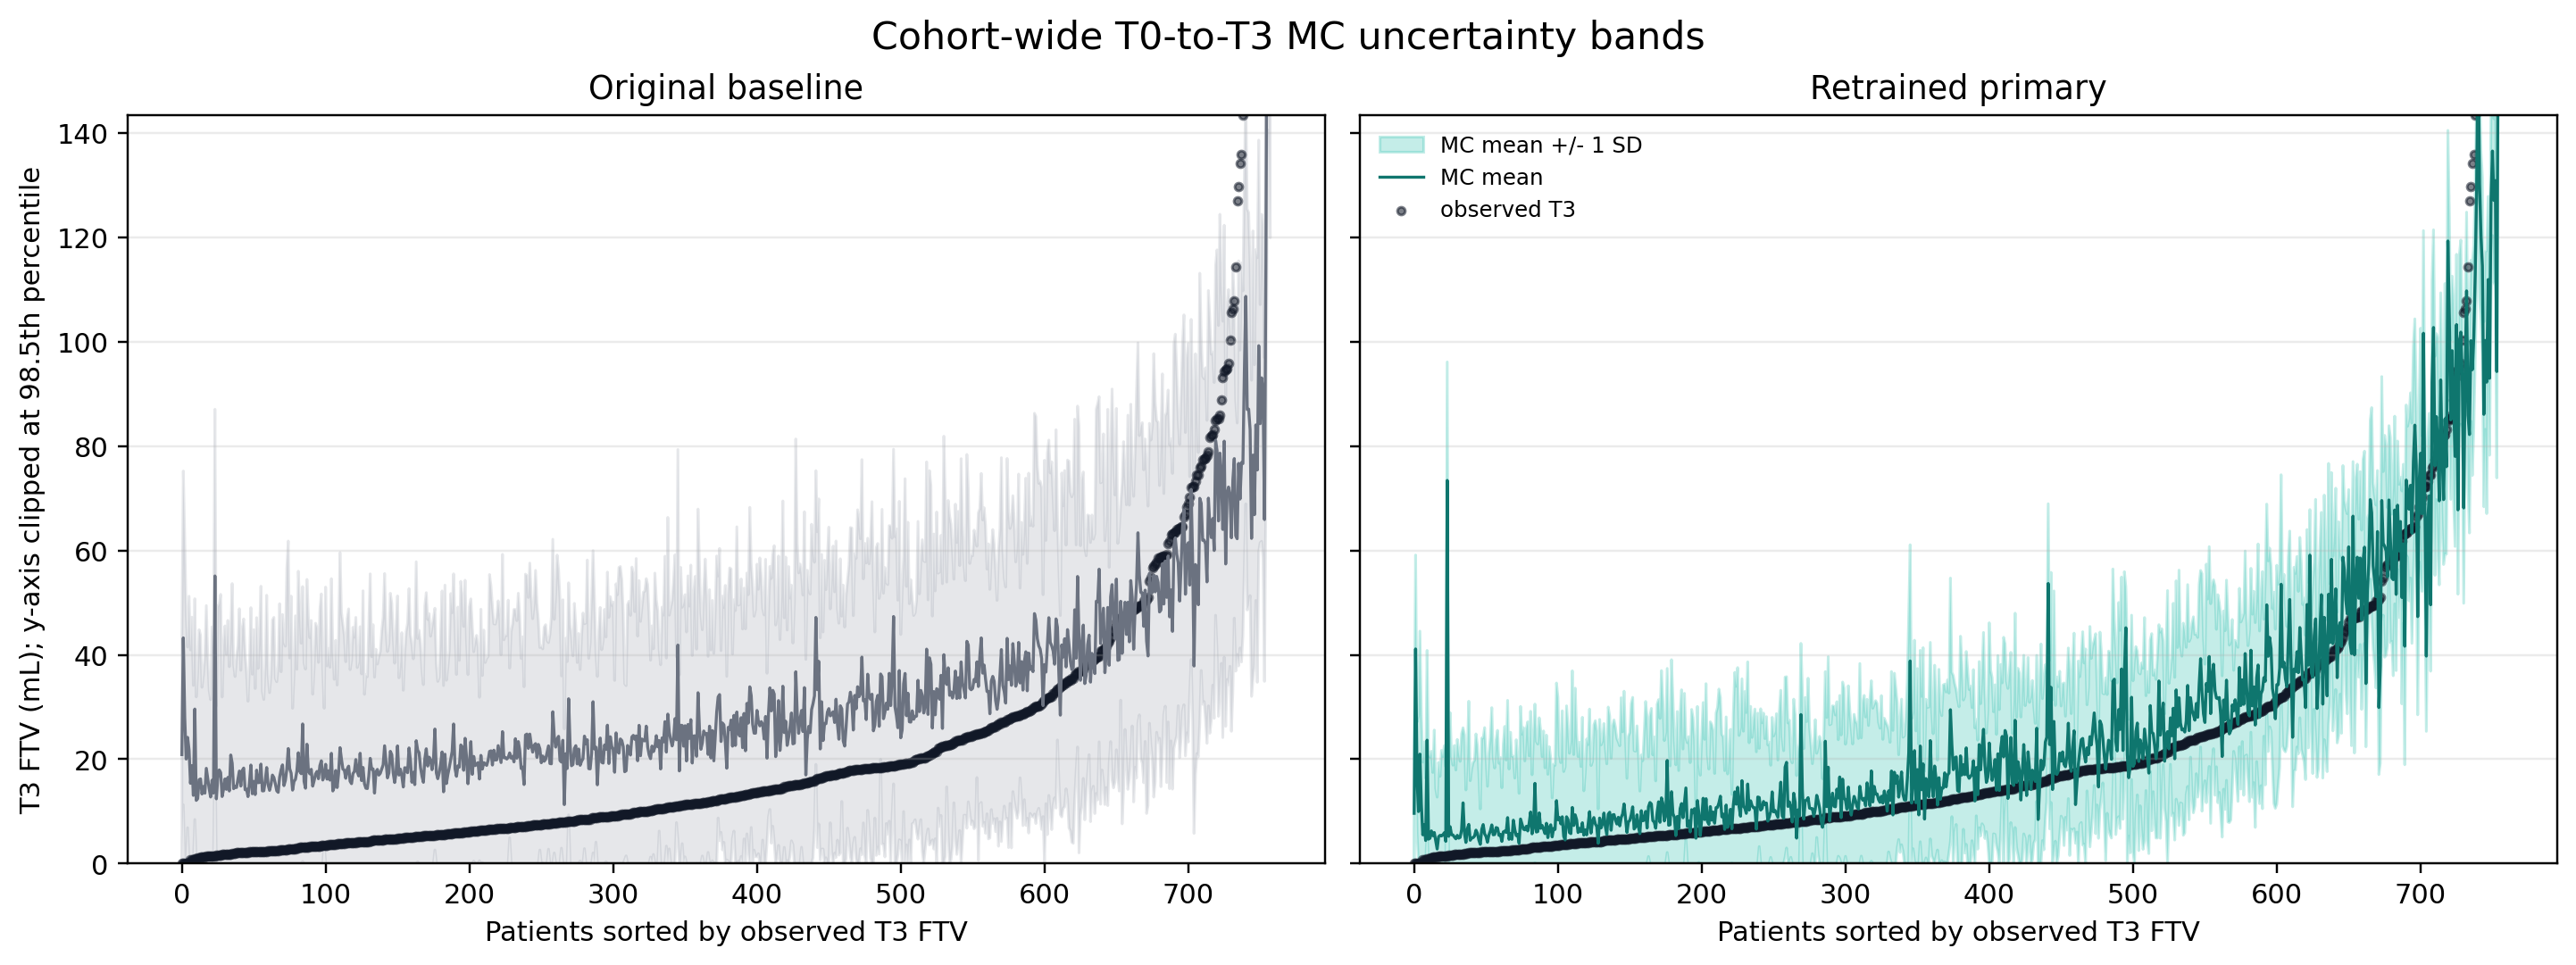
\includegraphics[width=0.88\textwidth]{figures/mc_t0t3_patient_uncertainty_sorted.png}
\caption{Cohort-wide \Tzero$\rightarrow$\Tthree{} MC uncertainty bands sorted
by observed final-visit FTV. The retained graph shifts MC means toward
observed burden and narrows the patient-level predictive bands relative to the
original graph rollout.}
\label{fig:uncertaintybands}
\end{figure*}

\subsection{Robustness, Transfer Stress Test, and Clinical Readouts}

The remaining analyses test whether this calibrated distribution remains stable
across conditioning horizons, source collections, burden strata, and
clinically interpretable MRI-burden thresholds.

The retained graph improvement persisted across conditioning horizons. MC-mean
FTV MAE was 5.56, 5.90, and 5.68 mL for \Tzero, \Tone, and \Ttwo{}
conditioning, with paired reductions versus the original graph rollout of
9.70, 8.97, and 8.13 mL. Source-stratified internal robustness was stable:
ACRIN-6698 had 4.55 mL MC-mean MAE and 0.881 raw coverage, while I-SPY2 had
5.93 mL MC-mean MAE and 0.876 raw coverage. In the small independent
Breast-MRI-NACT-Pilot stress test, \modeltag{} was best among the tested
graph-family variants but still overpredicted FTV, giving 15.01 mL MC-mean MAE
and 0.545 raw 90\% coverage. The value of this analysis is conservative:
without target-cohort residual recalibration, it tests whether model-family
ordering persists under collection shift and identifies recalibration as the
next validation step.

\begin{table}[t]
\centering
\caption{Compact robustness and boundary summary for the retained
\modeltag{} graph MC rollout. Conf. width is conformal 90\% interval width.
The NACT row is a transfer stress test with 11 graph-ready patients, not a
powered external validation cohort.}
\label{tab:robustness}
\scriptsize
\setlength{\tabcolsep}{2.8pt}
\begin{tabular}{lrrrrr}
\toprule
Check & $n$ & MC MAE & CRPS & Raw cov. & Conf. width \\
 & & (mL) & & & (mL) \\
\midrule
\Tzero$\rightarrow$\Tthree{} horizon & 758 & 5.56 & 4.00 & 0.877 & 22.38 \\
\Tone$\rightarrow$\Tthree{} horizon & 758 & 5.90 & 4.18 & 0.865 & 25.61 \\
\Ttwo$\rightarrow$\Tthree{} horizon & 758 & 5.68 & 3.94 & 0.860 & 24.45 \\
ACRIN-6698 source & 202 & 4.55 & 2.93 & 0.881 & 21.78 \\
I-SPY2 source & 556 & 5.93 & 4.39 & 0.876 & 22.59 \\
NACT external stress & 11 & 15.01 & -- & 0.545 & -- \\
Top 5\% \Tthree{} burden & 38 & 31.57 & -- & 0.237 & -- \\
\bottomrule
\end{tabular}
\end{table}

Burden-tail behavior is the main safety boundary exposed by the uncertainty
analysis. Below the top decile of observed \Tthree{} FTV, \modeltag{} reached
3.97 mL MC-mean MAE, 0.924 raw coverage, and 2.49 CRPS; in the top 5\% it
reached 31.57 mL MC-mean MAE and 0.237 raw coverage. Molecular subtype checks
showed improvement over the original graph rollout in every stratum, but the
HR-/HER2+ group was smallest and hardest ($n=57$, 7.52 mL MC-mean MAE).

\begin{figure*}[t]
\centering
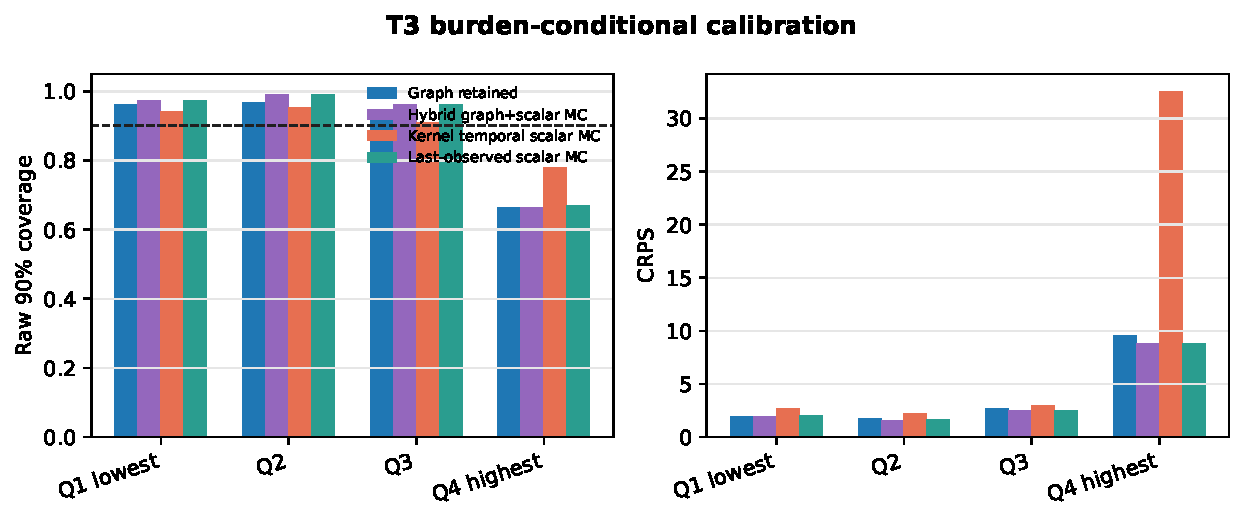
\includegraphics[width=0.86\textwidth]{figures/calibration_by_t3_burden.pdf}
\caption{Burden-conditional \Tzero$\rightarrow$\Tthree{} calibration by
observed final-visit FTV quartile. The retained graph distribution improves
over the original graph baseline but remains less calibrated in the
high-volume tail; scalar and hybrid readouts remain strong when only scalar
burden is required.}
\label{fig:burdencalibration}
\end{figure*}

The MC samples also support clinically interpretable MRI-burden readouts. For
low residual imaging burden, $P(\Tthree{}\,\mathrm{FTV}<5\ \mathrm{mL})$ gave
AUC 0.957, sensitivity 0.755, specificity 0.970, positive predictive value
0.870, and negative predictive value 0.937. For substantial residual burden,
$P(\Tthree{}\,\mathrm{FTV}>20\ \mathrm{mL})$ gave AUC 0.984, sensitivity
0.967, specificity 0.914, positive predictive value 0.844, and negative
predictive value 0.983. Last-observed FTV was similarly discriminative,
reinforcing that the added value of the graph framework is calibrated future
burden plus graph-native tumor-state forecasting.

\begin{table}[t]
\centering
\caption{Secondary MRI-burden threshold readouts for the retained MC samples.
These are imaging-burden scores, not pathology response probabilities.}
\label{tab:clinicalreadout}
\scriptsize
\setlength{\tabcolsep}{2.6pt}
\begin{tabular}{lrrrr}
\toprule
Readout & AUC & Sens. & Spec. & PPV/NPV \\
\midrule
$P(\Tthree{}\,\mathrm{FTV}<5)$ & 0.957 & 0.755 & 0.970 & 0.870/0.937 \\
Last FTV $<5$ mL & 0.961 & 0.679 & 0.980 & 0.900/0.920 \\
$P(\Tthree{}\,\mathrm{FTV}>20)$ & 0.984 & 0.967 & 0.914 & 0.844/0.983 \\
Last FTV $>20$ mL & 0.986 & 0.972 & 0.902 & 0.827/0.985 \\
\bottomrule
\end{tabular}
\end{table}

\begin{figure}[t]
\centering
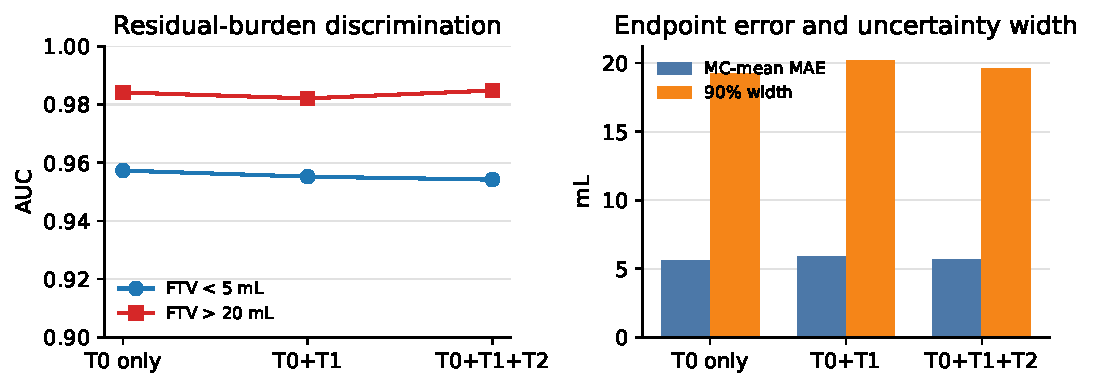
\includegraphics[width=\columnwidth]{figures/clinical_burden_monitoring_by_visit.pdf}
\caption{Serial MRI-burden monitoring readouts from the retained model. Low-
and high-burden discrimination remain high as additional MRI visits are used
for conditioning, while MC error and interval width summarize endpoint
uncertainty.}
\label{fig:clinicalmonitoring}
\end{figure}

\section{Discussion}
\label{sec:discussion}

The results support a layered interpretation of longitudinal tumor forecasting.
Graph message passing is valuable when local neighborhoods reveal response
structure that isolated node features only partially observe. Endpoint
calibration is separately necessary because a graph rollout can preserve
sampled-cloud geometry while remaining biased in total active burden. Residual
MC then converts the calibrated center into a patient-level distribution whose
coverage and sharpness can be evaluated directly.

The main result is therefore not a single model ranking. It is a modular
evaluation showing that graph dynamics, endpoint calibration, scalar readout
calibration, and residual uncertainty calibration have different roles. This
is why the scalar controls, transfer stress test, and tail analysis are part of
the evidence rather than secondary caveats.

For breast imaging, the most defensible use is uncertainty-aware MRI-burden
monitoring. Expected FTV summarizes likely residual enhancing burden; interval
width and coverage describe uncertainty; and MC threshold probabilities give
readouts such as low residual burden or substantial residual burden. These
outputs could support trial analytics or reader-facing response monitoring
after external validation, but they should not be interpreted as treatment
counterfactuals or pathology-response probabilities. The modest association of
the low-burden readout with pCR in available labels reinforces that boundary.

The scalar controls are deliberately strong and shape the claim. If the only
goal is scalar future FTV, last-observed or hybrid residual calibration is hard
to beat. This strengthens the modular interpretation: scalar readouts are
efficient for scalar endpoint forecasting, while the graph model supplies the
structured tumor state, active-node dynamics, and sampled-cloud geometry needed
for spatial monitoring.

The main limits are also explicit boundary conditions. The I-SPY2/ACRIN result
is an internal held-out-patient evaluation, and the Breast-MRI-NACT-Pilot
analysis is a small stress test rather than a powered external validation. The
high-volume tail is not hidden by aggregate calibration; it defines the current
safety boundary for clinical interpretation. Future work should test larger
independent cohorts, FTV-stratified and subtype-aware residual calibration,
explicit decomposition of spatial and scalar uncertainty, and prospective
studies of whether uncertainty-aware FTV trajectories change reader confidence
or trial-level response assessment.

\section{Conclusion}
\label{sec:conclusion}

Endpoint-calibrated spatial graph rollouts convert serial breast DCE-MRI tumor
graphs into probabilistic future FTV distributions while retaining a
graph-native tumor-state forecast. In held-out I-SPY2/ACRIN patients, the
retained \modeltag{} graph reduced deterministic FTV MAE from 12.88 to
4.63 mL, graph-based MC-mean FTV MAE from 15.26 to 5.56 mL, raw 90\% coverage
from 0.766 to 0.877, and conformal 90\% interval width from 59.51 to
22.38 mL. Scalar and hybrid controls remain strongest for scalar-only FTV, but
the graph model provides the structured spatial state needed for longitudinal
tumor-state forecasting. The central methodological result is that graph
dynamics, endpoint calibration, and residual uncertainty calibration are
separable layers that should be evaluated together.

\bibliographystyle{IEEEtran}
\bibliography{references}

\end{document}
